\section{System overview}
DCP operates more than a hundred sites across the developing world. The sites serve different needs and hence have different-sized equipment. Some of the sites are \textit{islanded} meaning that they do not have a grid connection, while others are connected to a larger grid. Grid-connected sites could feasibly become candidates for a control system in the future. The first pilot however, and hence this thesis, will only consider islanded systems. Specifically, the solution and analysis of this thesis will focus on Chiwoza which is a medium-scale system supporting a health facility in rural Malawi.\\

Chiwoza has a microgrid topology as shown in figure \ref{fig:system_topology}. The individual components are \todo{check break}
\begin{itemize}
    \item \textit{PV-modules}   -   The systems only source of power production through the photovoltaic effect outlined in section \ref{seq:pv_and_irradiance}. The core component of the module is the PV-panel consisting of several smaller PV-cells. As shown in equation \ref{eq:pv_efficency}, the PV-panel has an efficiency $\eta$ based on its area $A$ and test conditions $P_{STC}$ and $G_{STC}$. Several PV-panels may be connected in series as in \ref{fig:pv_serial} adding their voltage and forming a PV-string. Several PV-strings may form a parallel configuration known as a PV-array, shown in \ref{fig:pv_parallel},  adding together their current. Each PV-array has a charge controller controlling the production. Lastly, several PV-arrays may again be connected in parallel to form the PV-module shown in \ref{fig:system_topology}. The goal of the configuration is to achieve the highest power without breaking the constraints set by other equipment such as the charge controller. The PV-modules are ground mounted at an angle, $\rho$, with an orientation described by the azimuth, $\alpha$, determining the amount, type and timing of irradiance reflected onto the modules. These, and the other relevant parameters for the PV-panels at Chiwoza are listed in \autoref{tab:chiwoza_pv_param}.
    
    \item \textit{Charge Controller}   -   Between the PV-array and DC-bus there is the charge controller. The DC-bus requires a certain voltage to charge the battery and connect to the inverter. This may vary somewhat based on the inverter demand and battery state of charge. Furthermore, the power from the PV-array varies with the solar conditions. The charge controller needs to convert the voltage from the PV-panels to the voltage of the DC-bus. A simple charge controller force the PV-array to operate at the DC-bus voltage. As PV-panels have a rated power curve, this is inefficient and leads to large losses of potential power. More modern Maximum Power Point Tracking (MPPT) controllers finds and set the optimum voltage for the PV-array, allowing for the maximal power output. This is then converted into the voltage required for the DC-bus.\cite{Svarc2022-oh} The output from the charge controller will be limited by the maximum allowed voltage on the DC-Bus,$V^{MAX}_DC$, and the maximum current the charge controller can output $I^{MAX}_{CC}$. As mentioned earlier, if there are multiple charge controllers,$n_{CC}$, the currents are added together increasing the total power, $P^{MAX}_{CC}$, from the PV-module. The parameters for the charge controllers  at Chiwoza is listed in \autoref{tab:chiwoza_cc_param}.
    
    \item \textit{Battery module}   -   The battery module stores the power produced by the PV-modules. The batteries used for DCPs systems are mostly \textit{lithium iron phosphate} (LiFePo4) batteries, with a few exceptions using \textit{lead-acid} batteries. Key parameters for the battery is the energy capacity, $E$, which expresses how much charge a battery can deliver at a specific discharge rate at its nominal voltage, and the \textit{min SOC} which describes at which SOC level the battery is no longer supplying. For this thesis, the maximum charge and discharge power,$P_B$ which tells how much current can be continuously delivered at the nominal voltage is also of interest and found for Chiwoza in \autoref{tab:chiwoza_bat_param}.  
    
    \item \textit{DC-Bus}   -   The DC-bus connects the charge controller, the battery and the inverter. Its voltage, shown as $V^{MAX}_{DC}$ in \autoref{tab:chiwoza_cc_param} should remain stable.
    
    \item \textit{DC/AC inverter}   -   The inverter separates the DC and AC sides of the microgrid. It converts the power from the DC side to supply the AC power needed for the loads at the AC side. The inverter has a maximum power limit, $inv_{max}$ constrains the amount of power the DC side can supply. The inverter capacity and efficiency for Chiwoza are found in table \ref{tab:chiwoza_inv_param}. 
    
    \item \textit{Load}   -   The loads are all connected equipment and lighting consuming the power. All loads are on the AC-side of the inverter. The various loads that are connected at Chiwoza is found in \autoref{tab:loads_chiwoza}. These were found through the user survey described in \autoref{seq:user_survey}. There are loads supporting the purpose of the facility at the site, these are known as \textit{Purpose loads}, or in the case of Chiwoza, \textit{Medical Loads}. These include medical equipment, lighting etc. Other loads provides services besides the facility's purpose for staff and visitors at the facility. This might be sockets open for phone charging, cooking appliances etc. There are also other loads that support the facility's purpose indirectly. The water pump and heater are examples of these. \todo{clarify site/facility here}
\end{itemize}
The system installed at the site can be described as a hybrid, islanded microgrid with AC-load. Hybrid because the PV- and battery module can be seen as a hybrid power source. It is important to note that the parameters and models used in this thesis are greatly simplified. 



\begin{figure}
    \centering
    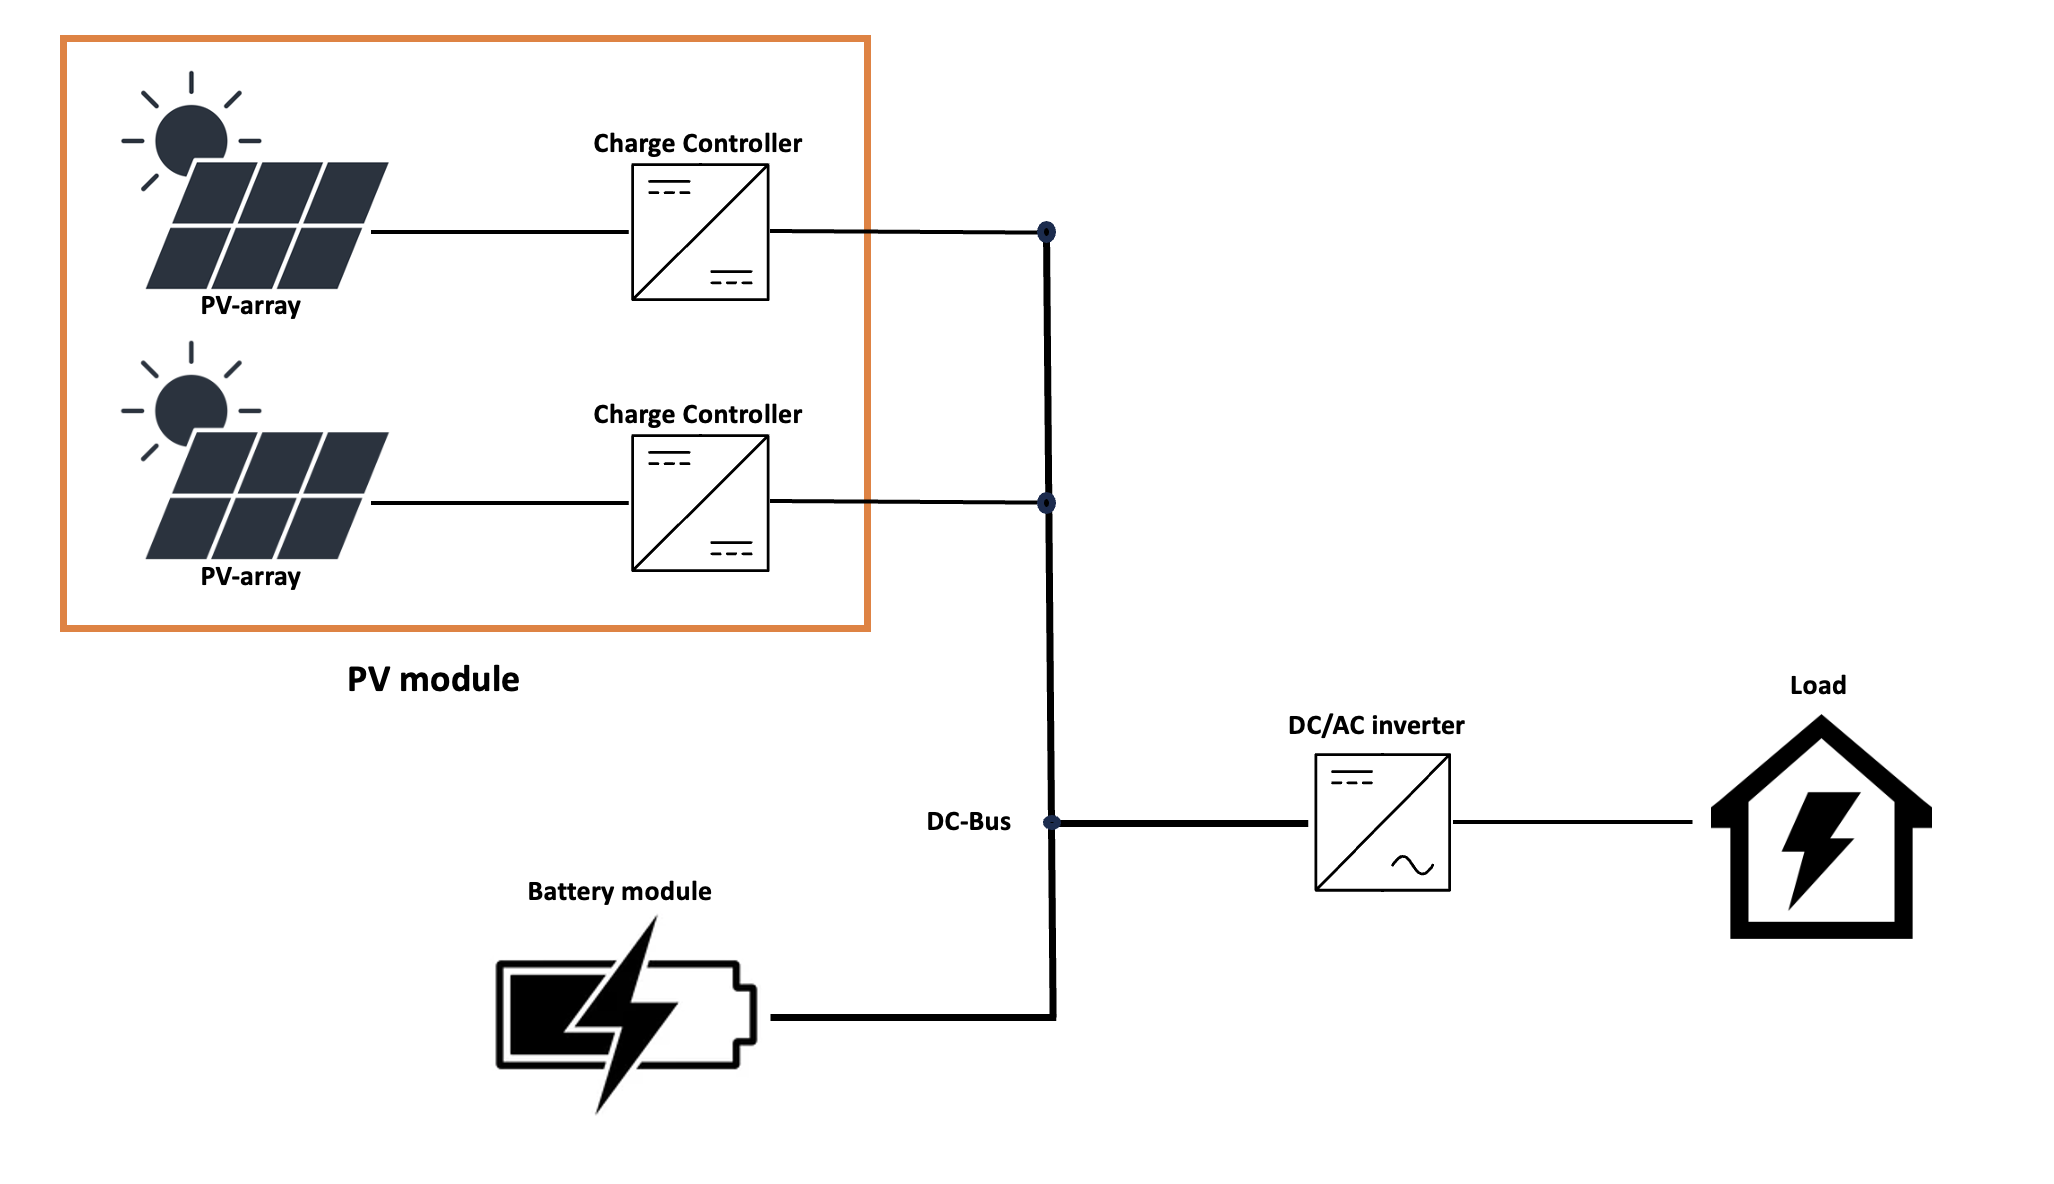
\includegraphics[width=\textwidth]{Figures/06SystemOverview/system_overview.png}
    \caption[Microgrid Topology]{Microgrid topology}
    \label{fig:system_topology}
\end{figure}

\begin{figure}
% First Subfigure
    \begin{subfigure}{\textwidth}
    \centering
    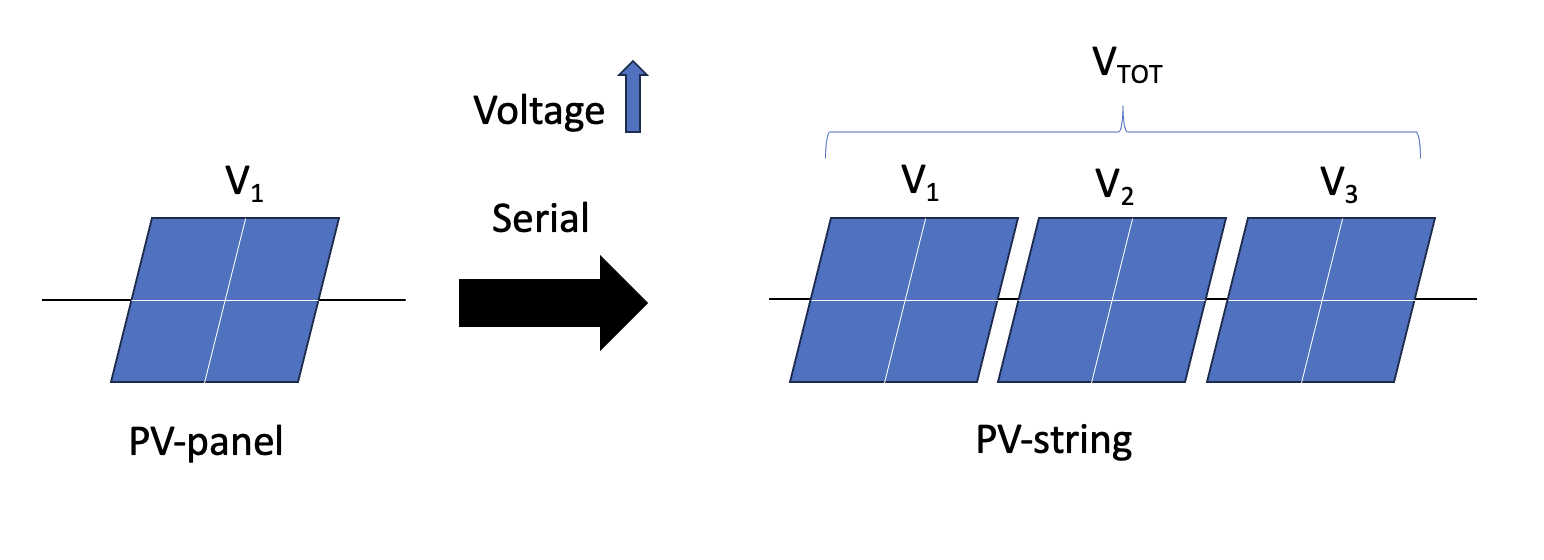
\includegraphics[width=\linewidth]{Figures/06SystemOverview/pv_serial.png}
    \caption[PV-serial]{PV-panels connected in serial forming an PV-string with increased voltage. $V_{TOT} = V_1 + V_2 + V_3$}
    \label{fig:pv_serial}
  \end{subfigure}

  % Add some vertical space between the subfigures
  \vspace{0.5cm}

  % Second Subfigure
  \begin{subfigure}{\textwidth}
    \centering
    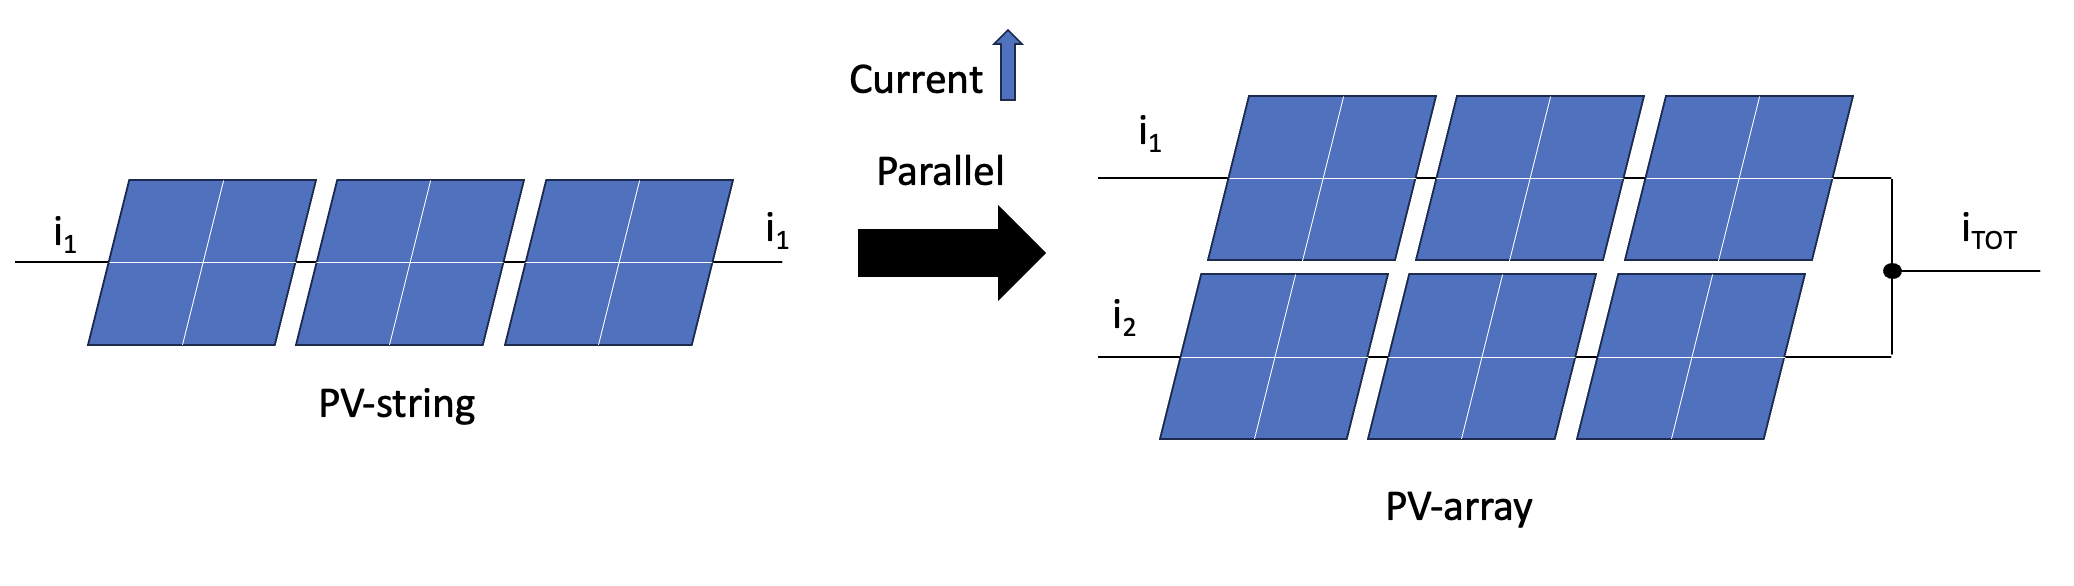
\includegraphics[width=\linewidth]{Figures/06SystemOverview/pv_parallel.png}
    \caption[PV-parallel]{PV-strings connected in parallel forming a PV-array with increased current. $i_{TOT} = i_1 + i_2$}
    \label{fig:pv_parallel}
  \end{subfigure}

  \caption[PV-configuration]{PV-configurations}
  \label{fig:pv_configuration}
\end{figure}

\begin{table}[]
    \centering
    \begin{tabular}{c|c|c|c|c|}
         $P_{STC}[W]$& $G_{STC}[W/m^2]$ & $n_{panels}$& $\rho$ & $\alpha$  \\
         \hline
         375 & 1000 & 25 & 20 & 180  \\
    \end{tabular}
    \caption[Chiwoza PV-parameters]{Chiwoza PV-parameters}
    \label{tab:chiwoza_pv_param}
\end{table}

\begin{table}[]
    \centering
    \begin{tabular}{c|c|c|c|c}
         $V^{MAX}_{DC}[V]$& $I^{MAX}_{CC}[Am]$ & $n_{CC}$ & $P^{MAX}_{CC}[W]$ & Peak Efficiency \\
         \hline
         48 & 60 & 2 & 5760 & 96\%\\
    \end{tabular}
    \caption[Chiwoza Charge Controller parameters]{Chiwoza Charge Controller parameters. The maximum power, $P^{MAX}_{CC}$ is for the two charge controllers combined.}
    \label{tab:chiwoza_cc_param}
\end{table}

\begin{table}[]
    \centering
    \begin{tabular}{c|c|c}
         $E[kWh]$& $P_B,Max[kW]$ &Min SOC\\
         \hline
         7.5 & 7.5 & 5\%\\
    \end{tabular}
    \caption[Chiwoza battery parameters]{Chiwoza battery parameters.}
    \label{tab:chiwoza_bat_param}
\end{table}

\begin{table}[]
    \centering
    \begin{tabular}{c|c}
         $P_{MAX}[kVA]$& Peak Efficiency\\
         \hline
         5 & 99\%\\
    \end{tabular}
    \caption[Chiwoza inverter parameters]{Chiwoza inverter parameters.}
    \label{tab:chiwoza_inv_param}
\end{table}

\begin{table}[ht]
    \centering
    \small % Optional: smaller font size
    \begin{tabularx}{\textwidth}{|X|X|c|}
         \textbf{Load Name} & \textbf{Circuit(s)} & \textbf{Group Abbreviation}\\
         \hline
         Light (Medical) & Medical Light & P1\\
         \hline
         Phone/Laptop Charging (Medical)   &  Staff Socket 3 & P2\\
         \hline
         Oxygen Concentrator & Medical Socket & P3\\
         \hline
         HIV diagnosis equipment & Medical Socket & P3\\
         \hline
         Sterilizer & Medical Socket & P3\\
         \hline
         Microscope & Medical Socket & P3\\
         \hline
         Refrigerator(Medical) & Medical Socket & P5\\
         \hline
         Light (Staff) & Staff Light 1-3, Guardian Shelter Light, Fence Light & S1\\
         \hline
         Phone/Laptop Charging  &  Staff Socket 3, Guardian Shelter Socket  & S2\\
         \hline
         Entertainment (TV,Radio) & Staff Socket 3, Guardian Shelter Socket & S3\\         
         \hline
         Refrigeration (Staff) & Staff Socket 3 & S4\\
         \hline
         Cooking appliances & Staff Socket 3 & S5\\
         \hline
         Water Heater & Water Heater & W1\\
         \hline
         Water Pump & Water Pump & W2\\
         \hline
         $\text{Rental Batteries}^*$ & Rental Battery & H1\\
         \hline
         $\text{Solar Maize Mill}^*$ & Solar Mill & H2
    \end{tabularx}
    \caption[Loads at Chiwoza]{Connected Loads Chiwoza with their circuit and grouping based on \autoref{tab:load_abbreviations}. The loads marked by $*$ are not connected, but planned to be connected as additional revenue-generating loads}
    \label{tab:loads_chiwoza}
\end{table}

\subsection{Measurement and Data logging}\label{seq:data_collection}
Production and load measurement is critical for the effective control and operation of all power systems, including microgrids. All of DCP sites are equipped with several measurement and data logging devices. These may be grouped as in table \ref{tab:measurement_devices}, which shows what each device measures, and what that measurement is used to estimate internally in the device.\\

The measurement from the inverter gives a broad overview of the power flow in the system. On the demand side, this can be further examined by the meters, which are mounted on every circuit. A meter measures the consumption of a load within a time frame. However, as already mentioned, several loads may be connected to the same circuit. The power measurement is only from the circuit, so it is not immediately possible to identify which loads are running based on the consumption measured.\\

Data has been gathered from the site starting from the the installation date of the systems. As the installation date varies between the systems, there are different amounts of historical data for each system. Furthermore, data gathering and operations in developing countries are prone to connectivity issues and tampering with equipment. This has in some instances yielded large gaps or improbable data. There has also been cases of mislabeling of meters, so that meters records consumption for another circuit than the one it is actually to. These issues may be grouped as \textit{data integrity} issues. Low data integrity complicates the analytics and control. Circuits with no recent data in the last 3 months are assumed to be disconnected and hence disregarded in this thesis. This includes Staff Sockets 1 and Staff Sockets 2. 


\begin{table}[h]
    \centering
    \begin{tabular}{c|c|c|c}
        \textbf{Where} & \textbf{Measurement} & \textbf{Estimates} & \textbf{Sample resolution}\\
        \hline
         Battery & Voltage & SOC & minutes\\ 
         \hline
         Smart Meter & Power & Consumption & 15 minutes - 1 hour\\
         \hline 
         Inverter & Power & Production & minutes
    \end{tabular}
    \caption[Measurement devices]{Measurement devices at the sites}
    \label{tab:measurement_devices}
\end{table}


\section{Control System currently in place}\label{seq:current_syst}
As the performance of the proposed solution will be compared against the current control system, an outline of the current control measures is a prerequisite. From the hardware manufacturer, two key control features is included to avoid damage to hardware. These are\todo{check break}
\begin{itemize}
    \item \textit{Inverter overload protection} -   An inverter have a max power capacity. This can be exceeded for a limited amount of time, but if it is exceeded for a prolonged duration, the inverter will shut down to avoid damage. 
    \item \textit{Battery discharge protection} -   As batteries might be damage by a complete discharge due to a high voltage drop, the battery will stop supplying power once it reaches about 5\% State of Charge
\end{itemize}

In addition to this, a battery health measure is implemented by DCP to avoid calendar degradation by prolonged periods at a high state of charge. The control measure, shown as a \textit{Finite State Machine (FSM)} in figure \ref{fig:current_battery_control_FSM}, blocks charging above 90\% SOC early in the day before allowing it to fully charge up during the afternoon. The benefits of this control is consistent with the theory from \ref{seq:battery_health}. The effects of this is shown in figure \ref{fig:battery_charge_control_current}. 

This control measure does not consider future solar production or consumption but is purely a function of the time of day. Similarly, certain high power loads, such as the water pump and water heater are given specific time slots to run, which are all placed during the day when there is normal PV-production. This is however also a purely rule-based control based solely on the time of day.

\begin{figure}[h]
    \centering
    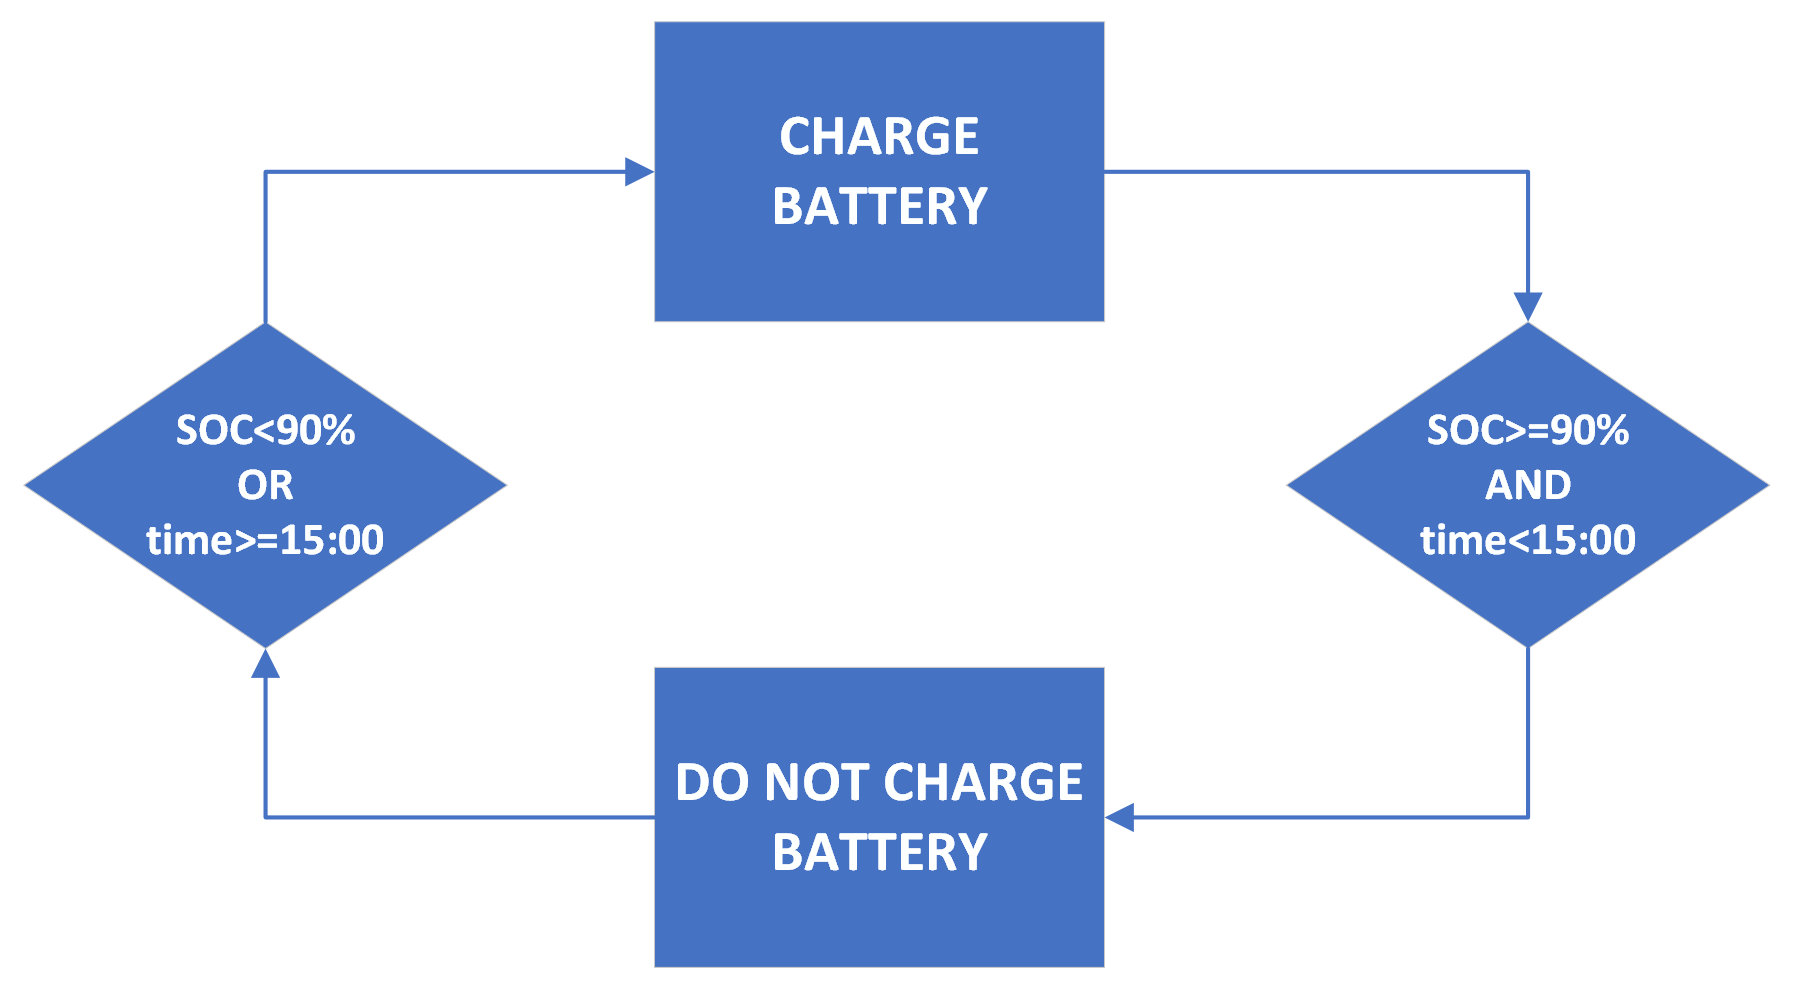
\includegraphics[width=\textwidth]{Figures/06SystemOverview/current_battery_control_FSM.png}
    \caption[Current Battery charge control system FSM]{Battery charge control measure currently in place as a FSM.}
    \label{fig:current_battery_control_FSM}
\end{figure}

\begin{figure}[h]
    \centering
    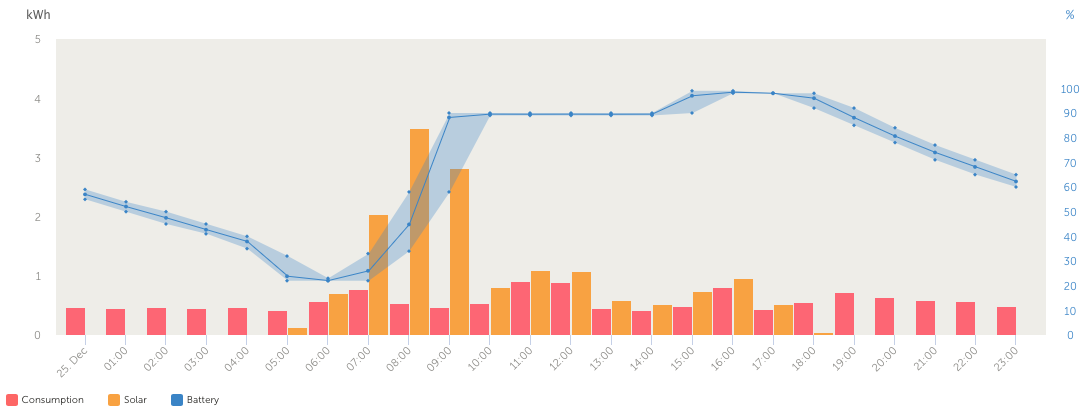
\includegraphics[width=\textwidth]{Figures/06SystemOverview/battery_charge_control_current.png}
    \caption[Current Battery charge control system]{Battery charge control measure currently in place. The picture is taken from DCPs monitoring system showing the operation on December 25th 2023.}
    \label{fig:battery_charge_control_current}
\end{figure}

\subsection{Weaknesses with current control system}\label{sec:weaknesses_current_syst}

\begin{figure}[h]
    \centering
    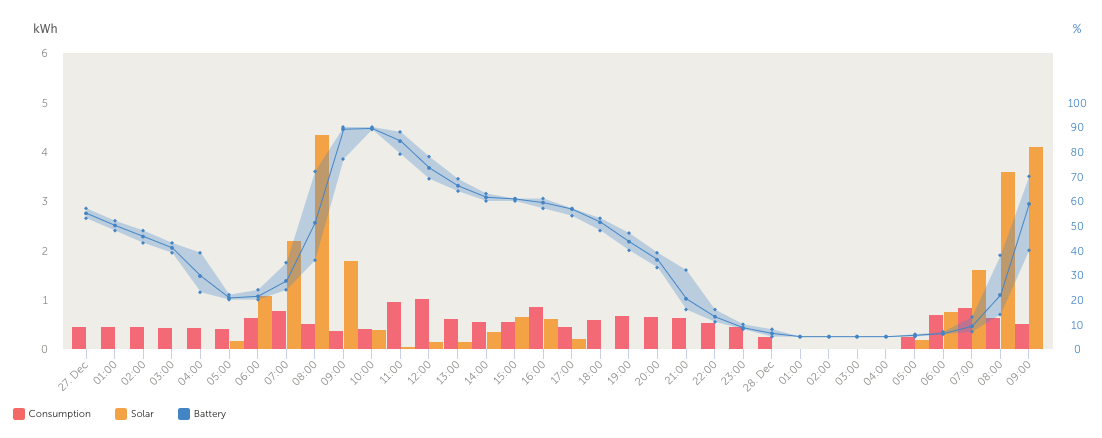
\includegraphics[width=\textwidth]{Figures/06SystemOverview/battery_charge_control_issue.png}
    \caption[Current control system weakness 1 - Battery Depletion]{Screenshot taken from DCPs monitoring platform. The yellow columns shows the production and the red the consumption during each hour. The battery SOC is the blue line.}
    \label{fig:battery_charge_control_issue}
\end{figure}

The two control action taken by DCP regarding the battery charging and time-control of high-power loads are reasonable during normal conditions. The inflexibility with regards to production and consumption conditions however, makes the current control system ill-equipped for days with poor production or high demand. Figure \ref{fig:battery_charge_control_issue} highlights this issue. The battery charge control policy described earlier curtails the charging of the battery after reaching 90\% early in the day, in expectation of being able to charge to remaining part during the afternoon. However, poor production during the afternoon inhibits the charging of the battery. As the battery does not reach its maximum state of charge, it is emptied early during the night. 

At sites with low consumption, there is an opposite problem. In section \ref{seq:battery_health} it was described how cycling the battery at a high state of charge was damaging to the battery. Some sites does not consume more than about 10\% of the battery capacity during nighttime. With the current control system, this will result in a battery cycle between 90-100\% SOC. In figure \ref{fig:battery_issues_high_cycling_chisuwi}, this pattern is shown for the site of Chisuwi, which has a low daily consumption. A more ideal charge cycle would either cycle between two lower values every day, or only charge a few times a week. The two weaknesses of the current control system can be summarized as an inability to adapt to changing conditions and different sites.

\begin{figure}[h]
    \centering
    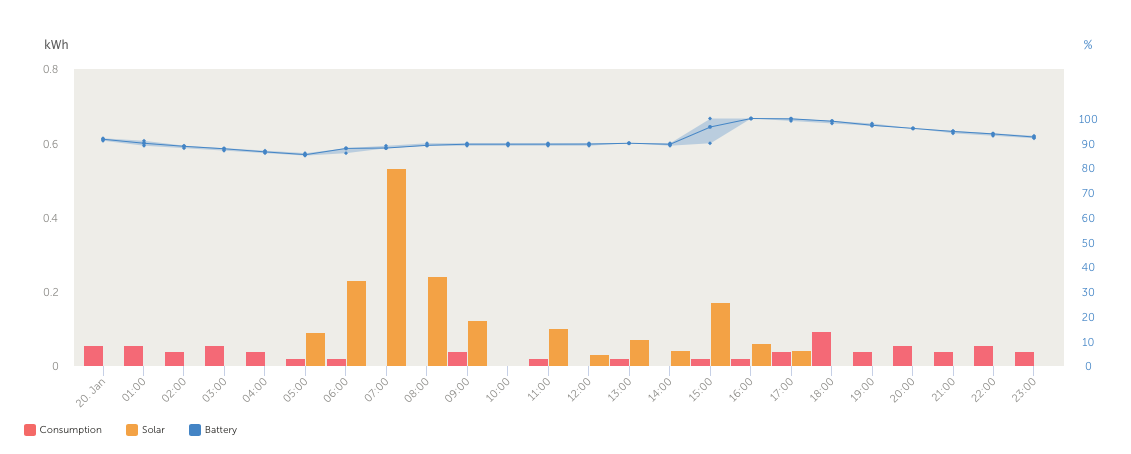
\includegraphics[width=\textwidth]{Figures/06SystemOverview/battery_issues_high_cycling_chisuwi.png}
    \caption[Current control system weakness 2 - High SOC cycling]{Screenshot taken from DCPs monitoring platform. The yellow columns shows the production and the red the consumption during each hour. The battery SOC is the blue line.}
    \label{fig:battery_issues_high_cycling_chisuwi}
\end{figure}
